\documentclass[12pt]{article}

\usepackage[english]{babel}

% Set page size and margins
\usepackage[a4paper,top=2cm,bottom=2cm,left=3.5cm,right=2cm,marginparwidth=1.75cm]{geometry}

\linespread{1.5}

% Useful packages
\usepackage{amsmath}
\usepackage{graphicx}
\usepackage[colorlinks=true, allcolors=blue]{hyperref}
\usepackage{caption}
\usepackage{ragged2e}

\usepackage{natbib}
\bibliographystyle{agsm}

%\usepackage[backend=biber,style=alphabetic,citestyle=mla]{biblatex}


%\addbibresource{sample.bib} %Imports bibliography file

%%%%%%%%%%%%%%%%%%%%%%%%%%%%%%%%%%%%%%%%%%%%%%%%%%%%%%%%%%%%%%%%%%%%%%%%%%%%%%%%%%%%%%%%%%%%%%%%%%%%%%%%%%%%%%%%%%%%%%%%
%% Document start
%%%%%%%%%%%%%%%%%%%%%%%%%%%%%%%%%%%%%%%%%%%%%%%%%%%%%%%%%%%%%%%%%%%%%%%%%%%%%%%%%%%%%%%%%%%%%%%%%%%%%%%%%%%%%%%%5

\title{Demand shocks and the labour share}
\author{Jamie Lenney}

\begin{document}
\maketitle

\begin{abstract}
Your abstract.
\end{abstract}

\section{Introduction}

The textbook sticky price New Keynesian model remains at the heart of modern economic policy analysis yet in recent years it's underlying transmission mechanism  has come under increasing criticism e.g. \cite{nekarda2020cyclical} or \cite{broer2020new}. In response to a demand shock, such as a monetary or fiscal tightening, the textbook sticky price models has markup's rise and redistributes income away from labour to capital. Consequently the labour share is pro-cyclical in response to demand shocks in these models, and at odds with the econometric evidence e.g. \cite{cantore2021missing} that robustly estimates the labour share as counter-cyclical to such shocks.

In this paper, based on the suggested framework of \cite{kaplan2020markups}, I analyse the introduction of an alternate non-production form of labour 'expansionary labour' into otherwise standard and popular business cycle models used for policy analysis. This form of labour is nested in the consumer facing sector and focuses on expanding the firms measure (variety) of goods available to customers as opposed to the labours more traditional role in the production of goods. I demonstrate the introduction of this form of labour delivers a counter-cyclical response of the labour share to demand shocks. As in the standard model, sticky prices combine with a fall in demand to raise markups as price do not fall enough to close the output gap. However, in a model with expansionary labour higher markups leads to higher demand for expansionary labour offsetting some of the fall in demand for production labour. In doing so the model can endogenously deliver a data consistent pro-cyclical response of labour productivity when hours are diverted to the less capital intensive consumer facing sector. The the also model weakens the link between markups and the level of profits as higher markups now redistribute income to expansionary labour as well as  capital.      

Given the focus of this analysis on the distribution of income and labour heterogeneity, I compare and contrast the transmission of demand shocks between the standard and augmented model under various levels of household heterogeneity. I find that..........[Results]

\subsection{Literature}

\begin{enumerate}
\item Labour share/transmission criticism
\item HANK
\item Intangibles/innovation
\item Overhead labour

\end{enumerate}
%\dots or bullet points \dots
%\begin{itemize}
%\item Like this,
%\item and like this.
%\end{itemize}


%%%%%%%%%%%%%%%%%%%%%%%%%%%%%%%%%%%%%%%%%%%%%%%%%%%%%%%%%%%%%%%%%%%%%%%%%%%%%%%%%%%%%%%%%%%%%%%%%%%%
%%%%%%%%%%%%%%%%%%%%%%%%%%%%%%%%%%%%%%%%%%%%%%%%%%%%%%%%%%%%%%%%%%%%%%%%%%%%%%%%%%%%%%%%%%%%%%%%%%%%%%

\section{Model}

The analysis is built around a standard medium scale closed economy New Keynesian model like that of \cite{smets2007shocks} or \cite{bayer2020shocks} in the case of heterogeneous households. All variants\footnote{Model parameters are as in table \ref{table:tabparam} unless otherwise stated.} of the model include sticky\footnote{Wages can be renegotiated and prices re-set subject to convex adjustment costs
} prices, wages, capital and investment adjustment costs. The labour market is organised around a labour union that aggregates labour services and sells them to firms. 

The government taxes labour, purchases final output and issues debt subject to fiscal rules that stabilise long run debt. The inflation targeting central bank set the nominal interest rate on government debt subject to a Taylor rule. 

Households maximise their lifetime utility subject to idiosyncratic productivity shocks, earn income through labour market participation and capital income from  returns to saving in liquid government bonds or an illiquid investment fund which owns the firms. 

There are two types of firms in the economy. Wholesale firms operate in a perfectly competitive market and sell their production to retail firms at marginal cost. Retail firms convert wholesale goods into numerous differentiated product lines over which they are monopolists and able to sell each line at a markup over marginal cost.  

\subsection{Firms}

\subsubsection{Wholesale firms}

A unit mass of wholesale firms $j$ produce under a Cobb Douglas production function by hiring production focused labour services $n_y$ and renting capital services $k_{j}$ based on solving the following maximisation problem in each period:

\begin{equation}
\Pi_{w,j}=Max_{y_{j},n_{j,y},k_{j}} \hspace{3mm} p_{w}y_{j}-w_{y}n_{y,j}-r_{k}k_{j}, \hspace{3mm} s.t. \hspace{3mm} y_{j}=z_{y} \left( k_{j}^{\alpha_{y}} n_{y,j}^{1-\alpha_{y}} \right)^{\theta_{y}}
\label{eqn:piw}
\end{equation}

This yields the following first order conditions: 

\begin{equation}
w_{y}=p_{w}\theta_{y}(1-\alpha_{y}) z_{y} k_{j}^{\alpha_{y}\theta_{y}} n_{y,j}^{(1-\alpha_{y})\theta_{y}-1} =     p_{w}\theta_{y}(1-\alpha_{y})\frac{y_{j}}{n_{y,j}}
\label{eq:firm1}
\end{equation}

\begin{equation}
r_{k}=p_{w}\theta_{y}\alpha_{y} z_{y} k_{j}^{\alpha_{y}\theta_{y}-1} n_{y,j}^{(1-\alpha_{y})\theta_{y}} =     p_{w}\theta_{y}\alpha_{y}\frac{y_{j}}{k_j}
\label{eq:firm2}
\end{equation}

In the symmetric equilibrium assuming perfect competition in the wholesale market price $p_{w}$ equals marginal cost $mc$. 

\subsubsection{Retail firms}

The major departure in this model from the literature is that of the retail firms problem. In each period retailers $j$ employ expansionary labour services $n_{e}$ and rent capital $k_{j}$ to manage  $M_{j}$ product lines $s$. Product lines are created by purchasing and differentiating homogeneous wholesale goods at the wholesale price. The retailers enjoy a monopoly on each product line and set the price $p_{s}$ subject to convex adjustment costs\footnote{For new products retailers assume the average economy wide price $P_{t-1}$ as a reference point for $p_{s,t}$.} $\Phi(.)$ and households demand elasticity $\epsilon_{p}$. Adopting the discount rate of their investors (the investment fund) the retail firms problem has the following form: \\


$\Pi_{r,j}=Max_{M_{j,t},n_{e,j,t},k_{j,t},\left\{p_{s,t},y_{s,t}\right\}} \hspace{3mm}\sum_{t=\tau}^{t=\infty} \frac{1+r_{a,\tau}}{p_{\tau} \prod_{z=\tau}^{z=t}(1+r_{a,z})}  \int_{0}^{M_{j,t}} (p_{s,t}-p_{w,t})y_{s,t} - \Phi(p_{s,t},p_{s,t-1}) ds$ \\ $-w_{e,t}n_{e,j,t}-r_{k,t}k_{j,t}, \hspace{3mm} $ \\

s.t. \hspace{3mm} $M_{j,t}=z_{e,t} \left( k_{j,t}^{\alpha_{e}} n_{e,j,t}^{1-\alpha_{e}} \right)^{\theta_{e}}$,
     \hspace{3mm} $y_{s,t}=\left( \frac{p_{s,t}}{P_{t}} \right) ^{-\epsilon_{p}}Y_{t} $ \\
\begin{equation}
\end{equation}
This yields the following first order conditions\footnote{Dropping the $t$ subscript where appropriate.}:

\begin{equation}
w_{e}=\Pi_{M_{j}}\theta_{e}(1-\alpha_{e}) z_{j} k_{j}^{\alpha_{e}\theta_{e}} n_{e,j}^{(1-\alpha_{e})\theta_{e}-1} =     \Pi_{M_{j}}\theta_{e}(1-\alpha_{e})\frac{M_{j}}{n_{e,j}}
\label{eq:firm3}
\end{equation}

\begin{equation}
r_{k}=\Pi_{M_{j}}\theta_{e}\alpha_{e} z_{j} k_{j}^{\alpha_{e}\theta_{e}-1} n_{e,j}^{(1-\alpha_{e})\theta_{e}} =     \Pi_{M_{j}}\theta_{e}\alpha_{e}\frac{M_{j}}{k_j}
\label{eq:firm4}
\end{equation}

 $0 = \frac{y_{s,t}}{P_{t}}-\phi\frac{1}{p_{s,t-1}}(\frac{p_{s,t}}{p_{s_t-1}}-1)Y_{t}  -\epsilon_{p} \frac{\Pi_{M_{s}}}{P_{t}y_{s,t}} \frac{p_{s,t}^{-\epsilon_{p}-1}}{P_{t}^{-\epsilon_{p}}}Y_{t} +        \phi\mathbf{E_{t}}\left[\frac{1}{1+r_{a,t+1}} \frac{p_{s,t+1}}{p_{s,t}^2}(\frac{p_{s,t+1}}{p_{s_t}}-1)Y_{t+1}\right]$
 \begin{equation}
 \label{eq:firm5}
\end{equation}
where $\Pi_{s}=y_{s}(p_{s}-p_{w})$ are the profits from product line $s$, $\left\{Y_{t},P_{t}\right\}$ is total economy output and prices and the functional form $\Phi_{t}=\frac{\phi}{2}(\frac{p_{s,t}}{p_{s_t-1}}-1)^2Y_{t} $ has been adopted for the price adjustment costs. 
In words the retail firms hire labour and rent capital up until the point the marginal profit from an extra product line equals the marginal cost of an extra input unit. Prices are adjusted to hit the firms target markup $\mu_{p}=\frac{\epsilon_p}{\epsilon_{p}-1}$ taking into account the present and future state of the economy. In the symmetric equilibrium where all firms choose the same price, and dropping higher order terms, equation \ref{eq:firm5} reduces to the familiar Philips curve around a zero inflation steady state:

\begin{equation}
    \pi_{t}=\frac{1}{1+r_{a,ss}}\mathbf{E}[\pi_{t+1}]+\frac{\epsilon_{p}-1}{\phi}\hat{mc}
    \label{eq:pc}
\end{equation}

where $\pi$ is retail price inflation and $\hat{mc}$ is the log deviation of marginal cost from steady state. 

\subsection{Investment fund}

As in \cite{kaplan2018monetary} households can pay into an investment funds which owns and rents out the capital stock $K$ as well as the shares of all firms $X$, and receives rental payments $r_{k}$ and dividends $\Pi_{d}$. The investment fund objectives is to invest in capital and shares to maximize it's value subject to rate of return $r_a$ and investment adjustment costs $\Psi(.)$:\\


$A_{\tau}=Max_{I_{t},K_{t},X_{t}}\sum_{t=\tau}^{\infty}  \frac{1+r_{a,\tau}}{\prod_{z=\tau}^{z=t}(1+r_{a,z})}  
\left( r_{k,t} K_{t-1}+\Pi_{d,t}*X_{t-1}+q_{s,t}(X_{t-1}-X_{t}) - I_{t} - \Psi(I_{t}) \right)$ \\
s.t. \hspace{3mm} $K_{t}=(1-\delta)K_{t-1}+I_{t}$ \\
\begin{equation}\label{eq:fundvalue}
\end{equation}

Equation \ref{eq:fundvalue} tells us that the funds value is the present discounted value of future dividends minus the costs of investments in capital and stocks at price stockprice $q_s$. Assuming a functional form of $\Psi(I_{t})=\frac{\Delta}{2}log(\frac{I_t}{I_{t-1}})^2I_{t}$ and denoting the shadow value of capital $q_k$, yields the following first order conditions for the investment funds problem:

%$\Psi(I_{t})=\frac{\Delta}{2}(\frac{I_{t}}{K_{t-1}}-\delta)^2K_{t-1}$
\begin{equation}
    1+r_{a,t+1}=\mathbf{E}\left[\frac{q_{s,t+1}+\Pi_{d,t+1}}{q_{s,t}}\right]
    \label{eq:inv1}
\end{equation}

\begin{equation}
%q_{k,t}=1+\Delta(\frac{I_{t}}{K_{t-1}}-\delta)
q_{k,t}=1+\Delta log(\frac{I_t}{I_{t-1}})+\frac{\Delta}{2}log(\frac{I_t}{I_{t-1}})^2- \mathbf{E}\left[\frac{\Delta}{1+r_{a,t+1}}\frac{I_{t+1}}{I_{t}}log(\frac{I_{t+1}}{I_{t}})\right]
\label{eq:inv2}
\end{equation}

\begin{equation}
%q_{k,t}=\mathbf{E}\left[\frac{1}{1+r_{a,t+1}} \left(r_{k,t+1}+(1-\delta)q_{k,t+1} %-\frac{\Delta}{2}(\frac{I_{t+1}}{K_{t}}-\delta)^2 + \Delta\frac{I_{t+1}}{K_{t}}(\frac{I_{t+1}}{K_{t}}-\delta) \right) 
%\right]
q_{k,t}=\mathbf{E}\left[\frac{r_{k,t+1}+(1-\delta)q_{k,t+1}}{1+r_{a,t+1}}\right] 
\label{eq:inv3}
\end{equation}

The investment fund therefore invests in capital and stocks in each period up until the expected returns are equalised. The value of the investment fund in each period is given by $A=q_{s}X+q_{k}K$, where X is the total amount of shares issued\footnote{I normalise X equal to 1}. 

\subsection{Government}

The government is composed of a fiscal authority and central bank. The government purchases final output funded through taxation and borrowing according to the following budget constraint. 

\begin{equation}
    B_{t}=\frac{1+r_{b,t-1}}{1+\pi_{t}}B_{t-1}+G_{t}-T_{t}
    \label{eq:gov1}
\end{equation}

where tax revenues are funded by a proportional tax $\tau_{t}$ on labour income. The government targets a constant level of purchases $G$ as percent of steady state output $Y_{ss}$. In order to accommodate this policy it adjusts the tax rate according to the following rule:

\begin{equation}
    \frac{\tau}{\tau_{ss}}=\frac{\tau}{\tau_{ss}}^{\rho_{\tau}}\frac{B_{t}}{B_{ss}}^{\gamma_{\tau_{B}}(1-\rho_\tau)}\frac{Y_{t}}{Y^{*}}^{\gamma_{\tau_{y}}(1-\rho_\tau)}
    \label{eq:gov2}
\end{equation}

which ensures long run debt stability but allows the deficit to adjust in the short run in response to the output gap\footnote{The output gap is defined in this model as the difference between period output $Y_{t}$ and what output would be under flexible prices and wages $Y^{*}$.}. The central bank smoothly adjusts the nominal interest on government bonds $r_{b}$ to hit it's inflation target according to a Taylor rule that also takes into account the output gap. 

\begin{equation}
    r_{b,t}=\rho_{r}r_{b,t-1}+(1-\rho_{r})(r_{b}^{*}+\gamma_{\pi}(\pi_{t}-\pi^*)+\gamma_{y}log(\frac{Y_{t}}{Y^{*}}))+\epsilon_{r,t}
\label{eq:gov3}
\end{equation}

\subsection{Household}

\subsubsection{Portfolio choice}

The household problem closely follows that of \cite{bayer2019precautionary}. Households seek to maximise their lifetime utility through consumption $c$\footnote{Here c is the composite of over the measure of product lines such that $c=\left(\int_{0}^M c_{j}^{\frac{\epsilon_{p}-1}{\epsilon_{p}}}dj\right)^{\frac{\epsilon_{p}}{\epsilon_{p}-1}}$ from which we can derive the demand for each product line as $c_{s}=\left( \frac{p_{s}}{P} \right) ^{-\epsilon_{p}}C $.} and the compliment of work (leisure) $h^c$. Households can self-insure themselves against idiosyncratic income risk by saving in liquid government bonds $b$ or the illiquid investment fund $a$. Illiquidity is captured in a Calvo like fashion by assuming that households can only adjust their holdings in the investment fund with some probability $\omega$ in each period.  

The household problem can be summarised by two Bellman equations that depend on a GHH preference based utilty function ((\cite{greenwood1988investment}), idiosyncratic states $(a,b,z,s)$ and the aggregate state of the economy $\lambda$:
\\

$    V_{adj}(b,a,z,s,\lambda)=Max_{a',b'} \hspace{2mm} \frac{1}{1-\sigma}(c-\frac{\kappa}{1+\psi}h^{1+\psi})^{1-\sigma} + \beta [ (\omega V_{adj}(b',a',h',s',\lambda')+ $ \\      $+ (1-\omega) V_{nadj}(b',a',z',s',\lambda')]$
\begin{equation}
\label{eq:Bellman1}
\end{equation}

$    V_{nadj}(b,a,z,s,\lambda)=Max_{b'} \hspace{2mm} \frac{1}{1-\sigma}(c-\frac{\kappa}{1+\psi}h^{1+\psi})^{1-\sigma} + \beta [ \omega V_{adj}(b',a,z',s',\lambda')+ $ \\      $+ (1-\omega) V_{nadj}(b',a,z',s',\lambda')]$
\begin{equation}
\label{eq:Bellman2}
\end{equation}

Subject to the constraints:

$    a'+b'+c=(1-\tau)w_{s}hz+a(1+r_{a})+\frac{1+r_{b}+\mathbf{1_{b<0}} \bar{r}}{1+\pi}b$, \hspace{2mm} $b \ge -\bar{B}$, \hspace{2mm} $a \ge 0$ \\

Households can only borrow in the liquid funds market up to an amount $\bar{B}$ and pay a penalty rate\footnote{ The revenue from the higher borrowing rate is assumeed to be lost through intermediation costs and therefore does not enter the government budget constraint. } above the risk free rate of $\Bar{r}$ when they do.

Labour income is composed of the aggregate sector wage $w_{s}$, aggregate hours $h$ and the persons individual productivity $z$. Individual productivity is subject to a stochastic AR(1) process such that:

\begin{equation}
    ln(z')=\rho_{z}ln(z)+\epsilon_{z}, \hspace{5mm} \epsilon_{z} \sim N(0,\sigma_{z}^2) 
\end{equation}

There is also a rare superstar state $\bar{z}$ (e.g. \cite{castaneda2003accounting}) that household transition to with low probability. This state captures households in the top 1 percent of the income distribution and helps deliver realistic wealth and income inequality. \\

The household problem can be boiled down and solved using the following Euler equations for the unconstrained households: \\

$\left(x_{adj}(a,b,z,\lambda)\right)^{-\sigma}=\beta\ \mathbf{E} \left[ \omega (1+r_{a}') \left( x_{adj}(a',b',z',\lambda' ) \right)^{-\sigma}+(1-\omega)\frac{dV_{nadj}(a',b',z',s',\lambda)}{da} \right]$
\begin{equation}
\end{equation}
$\left(x_{adj}(a,b,z,s,\lambda)\right)^{-\sigma}=\beta\ \mathbf{E} \left[ \omega \frac{1+r_{b}'}{1+\pi'} \left( x_{adj}(a',b',z',s',\lambda') \right)^{-\sigma}+(1-\omega)\frac{1+r_{b}'}{1+\pi'}\left( x_{nadj}(a',b',z',s',\lambda') \right)^{-\sigma} \right]$
\begin{equation}
\end{equation}
$\left(x_{nadj}(a,b,z,s,\lambda)\right)^{-\sigma}=\beta\ \mathbf{E} \left[ \omega \frac{1+r_{b}'}{1+\pi'} \left( x_{adj}(a,b',z',s',\lambda) \right)^{-\sigma}+(1-\omega)\frac{1+r_{b}'}{1+\pi'}\left( x_{nadj}(a,b',z',s',\lambda') \right)^{-\sigma} \right]$
\begin{equation}
\end{equation}

where $x_{adj/nadj}$ is the household choice of $c-\frac{\kappa}{1+\psi}h^{1+\psi}$ in the adjustment or non-adjustment case.

\subsubsection{Aggregate wages and  labour supply} 

Households rely on labour unions to negotiate hours/wages on their behalf as in \cite{schmitt2005optimal}. There is a continuum of labour unions, each with a monopoly over the labour services it sells to firms in each sector. Labour unions negotiate on the basis of their members average utility subject to convex adjustments costs. Demand for the labour unions services $i$ in sector $s$ at time $t$ is given by:

\begin{equation}
    h_{i,s,t}=(\frac{w_{i,s,t}}{w_{s,t}})^{-\epsilon_{W}}
    \label{eq:union}
\end{equation}

In the symmetric equilibrium the labour unions optimisation problem simplifies after linearisation to the following and standard wage Phillips curve in each sector:

\begin{equation}
    \pi_{w,s,t}=\beta \mathbf{E_{t}}[\pi_{w,s,t+1}] - \frac{(1-\tau_{t})(\epsilon_{w}-1)}{\phi_{w}}\hat{\mu_{w}}
\end{equation}

where under GHH preferences,  $\hat{\mu_{w}}=\hat{w_{t}}  - \hat{p_{t}} -\psi \hat{h_t}$ is the log deviation from steady state of households marginal rate of substitution between consumption and leisure. 

\subsection{Equilibrium}

Equilibrium in the model is above is characterised by a set of value functions $\left\{V_{adj},V_{nadj} \right\}_{t}$, household policy functions $\left\{x_{adj},x_{nadj},b'_{adj},b'_{nadj},a'_{adj}  \right\}_{t}$,  quantities $\left\{N_{y},N_{e},M,y,K,B,A,G\right\}_{t}$, set of prices $\left\{w_{y},w_{e},\pi,\pi_{w,e},\pi_{w,y},r_{b},r_{a},q_{k},q_{s},r_{k},\tau_{t} \right\}_{t}$, stochastic states $\left\{z_{e},z_{y} \right\}_{t}$ and an aggregate distribution over $(a,b,z)$ $\left\{\chi \right\}_{t}$ such that:

\begin{enumerate}
    \item The household policy functions solve the household planning  problem (eq \ref{eq:Bellman1} and \ref{eq:Bellman2}) given period t prices and expected $t+1$ prices.
    \item Firms profit maximise such that equations \ref{eq:firm1}, \ref{eq:firm2}, \ref{eq:firm3}, \ref{eq:firm4} and \ref{eq:pc} hold in each period. 
    \item The investment fund maximises it's value in accordance with equations \ref{eq:inv1} - \ref{eq:inv3}. 
    \item Unions negotiate wages such that the wage philips equations hold (eq. \ref{eq:union}). 
    \item The market for government bonds $B$ and the investment fund clears in each period. i.e. $A_{t}=\int_{i}a_{t}'di$ and $B_{t}=\int_{i}b_{t}'di$ and the aggregate distribution $\chi_{t}$ evolves according to the household policy functions and the stochastic process $z$. 
    \item The government budget constraint holds (eq. \ref{eq:gov1}) and government follows it's fiscal and monetary rules (eq. \ref{eq:gov2} and \ref{eq:gov3}). 
    \item Stochastic TFP processes $z_{e},z_{y}$ follow stationary AR1 processes. 
\end{enumerate}

In the subsequent sections we shall study the dynamics of the generalised model laid out above in three principle settings:  

\begin{enumerate}
    \item \textbf{RANK} In the RANK equilibrium households fully insure each other such that consumption and labour is the same between households. Free movement of labour and capital between sectors equates $w_{y}=w_{e}$. Therefore this models boils down to the textbook medium scale closed economy New Keynesian model with the exception of role of expansionary labour in the retail sector. 
    \item \textbf{WCNK} In this setting households are one of two types, workers or capitalists as in e.g. \cite{broer2020new}. Capitalists do not work but instead derive income from capital rental income and monopolistic profits. For tractability as in \cite{ravn2021macroeconomic} I assume $\bar{B}=0$ and net zero issuance of government bonds $B$ in each period such that the wealth distribution in the economy is degenerate. This means that the interest rate on government bond's adjusts such that the highest productivity households $\bar{z}$ consumes all of their income and by extension the  lower productivity households $z<\bar{z}$ do so as well  due to the borrowing constraint. Again free movement of labour and capital between sectors equates $w_{y}=w_{e}$.    
    \item \textbf{HANK} In this setting households must self insure against idiosyncratic income risk using liquid and illiquid assets producing a rich non-degenerate wealth distribution as in \cite{bayer2020shocks}. I also consider the case where workers idiosyncratic state include their sector $y/n$ and drop free movement of workers between sectors.   
\end{enumerate}


%%%%%%%%%%%%%%%%%%%%%%%%%%%%%%%%%%%%%%%%%%%%%%%%%%%%%%%%%%%%%%%%%%%%%%%%%%%%%%%%%%%%%%%%%%%%%%%%%%%%
%%%%%%%%%%%%%%%%%%%%%%%%%%%%%%%%%%%%%%%%%%%%%%%%%%%%%%%%%%%%%%%%%%%%%%%%%%%%%%%%%%%%%%%%%%%%%%%%%%%%%%

\section{The labour share and demand shocks}

The labour share in the symmetric equilibrium of the model is defined as $\frac{w_{y}l_{y}M+w_{e}l_{e}}{pY}$. Where in the equilibrium M product lines are sold by all retailers such that total production labour services demand is $M l_{y}$ and total output is $Y=M y$. Substituting for the first order conditions for $w_e,w_y$ yields the following expression for the labour share:

\begin{equation}\label{eq:labour share}
    \frac{p_{w} \frac{dy}{d l_{y}} l_{y}M  +y(p-p_w)\frac{dM}{d l_{e}}l_{e} }{pMy} = \frac{1}{\mu_p} \xi_{y,l_{y}} + (1-\frac{1}{\mu_p})\xi_{M,l_{e}}
\end{equation}

where we've also made used of the fact that the retail markup is $\mu_{p}=\frac{p}{p_w}$. Equation \ref{eq:labour share} shows that the labour share in the model is pinned down by an inverse markup weighted average of the elasticity of labour in each of the sectors. For the particular Cobb Douglas framework of section 2 and using equations \ref{eq:firm1} and \ref{eq:firm3} this can be rewritten as:

\begin{equation}\label{eq:labour share2}
    s_l= \frac{1}{\mu_p} \theta_{y} (1-\alpha_{y}) + (1-\frac{1}{\mu_p})\theta_{e}(1-\alpha_{e})
\end{equation}

 In the textbook New Keynesian model the labour share is simply the left hand side term. The right hand side term accounts for the fact that labour now contributes by expanding the measure of goods $M$ on offer. Therefore for a given markup the labour share is strictly larger in the model with expansionary labour which provides a useful break to the relationship between markups and the overall labour share as markups now need to cover the cost of expansionary labour. Now consider the derivative of the labour share with respect to the markup: 

\begin{equation}
    \frac{d s_l}{d\mu}=-\frac{1}{\mu_p^2} \theta_{y} (1-\alpha_{y}) +\frac{1}{\mu_p^2}\theta_{e}(1-\alpha_{e})
\end{equation}

This shows the direction in which the labour share moves in response to a change in the markup is pinned down by the relative returns to scale of labour in the two sectors. Therefore in the framework of section 2 it suffices to set $\theta_{e}(1-\alpha_{e}) > \theta_{y}(1-\alpha_{y}) $ to create a positive correlation between movements in the markup and the labour share, or negative\footnote{In the New Keynesian model pricing frictions prevent firms from adjusting prices immediately to their target markup. For example in the face of a negative demand shock, production costs fall due to a decline in demand for the factors of production. This causes the markup to rise as prices do not fall 1 for 1 with marginal costs.} correlation between the output gap and the labour share. The intuition for this is rising markups cause a substitution away from production labour and towards expansionary labour. This put more weight on expansionary labour in the overall labour share calculation, and if returns to scale are higher for expansionary labour, then this will raise the entire economy labour share because the labour share is a weighted average of returns to scale over the two sectors. 

Turning to the response of productivity. The textbook New Keynesian model  with decreasing returns to scale in labour has an unambiguous rise in productivity in response to negative demand shocks\footnote{Consider for example the derivative with respect to N of productivity in Cobb Douglas production framework with $\frac{d}{dN} \left(\frac{Y}{N}\right) =-\alpha K^{\alpha}N^{-(1+\alpha)} <0$.}. In the model with expansionary labour this need no longer be the case. The reason for this is the rise in productivity from the decline in employment in the production sector is now offset by a rise in employment in the expansionary sector. This rise in employment in the expansionary sector reduces productivity in that sector and the overall fall in employment. As we see in figures \ref{fig:IRF_RANK} - \ref{fig:IRF_HANK}  this offsetting effect dominates creating a data consistent positive correlation between productivity and the output gap. 

Finally a word on intuition. The important distinction in terms of the model is that some workers contribute to expanding the measures of goods on offer where as others produce those goods. As already discussed there are numerous categories one might think of as falling under the header of expansionary such as R\&D or marketing. It could also be reasonably argued that the share of labour in these activities is higher than that of production activities which will be more reliant on capital and routine tasks.
One could consider the division of expansionary and production labour along a task based instead of sector or role based dimension. For example individual workers might divide their time between product development and production of existing goods and services. In the face of a negative demand shock, where demand for existing product lines falls it would seem optimal to devote more time to expansionary activities. However a task based version of the above framework while still supporting this optimal shift to expansionary activities would not deliver the desired counter-cyclical movement in the labour share. One can verify\footnote{See the appendix of \cite{kaplan2020markups}.} that in a one sector model, where production and expansionary activities occur within the same sector, firms will internalise the fact that expansionary activity leads to increased cost pressures on preexisting production activities. Firms will therefore allocate labour in such a way that the benefits of the rise in markups continue to result in a higher capital share. Therefore key to this mechanism is some friction that prevents firms from internalising this trade off.  


\section{Impulse response to a demand shock}

In this section we consider the response of the economy to a demand shock proxied by a monetary\footnote{The analysis is robust to other types of demand shocks such as government spending shocks or risk premium shocks produce similar results.} policy shock and focus on movement of the labour share and dampening/amplification of major economy aggregates in response to the shock in the model with expansionary labour in the retail sector relative to one without expansionary labour in the sector. 


\subsubsection{Calibration and computation}

The impulse response function to the monetary shock is computed at a quarterly frequency using the perturbation method of \cite{schmitt2004solving} around the models deterministic steady state up to first order. This requires expressing the model in SGU form:
\begin{equation}
\mathbf{E}\left[F(X_{ss},X'(X_{ss}),Y(X_{ss}),Y'(X'))\right]=0
\label{eq:sgu1}
\end{equation}
\begin{equation}
\mathbf{E}\left[F_{X_{|X=X_{SS}}}(X,X'(X),Y(X),Y'(X'))\right]=0
\label{eq:sgu2}
\end{equation}

and solving for the policy functions $Y(X)$ such that the above holds. Here $X$ are the models state variables and $Y$ the control variables. In the RANK and WNNK case this a relatively undemanding and well understood solution method. In the HANK case the dimensionality of the problem quickly become infeasible as the state vector X includes the entire wealth distribution. 

In order to simplify the problem I follow the procedures of \cite{bayer2020solving} who demonstrate the dynamics of these high dimension heterogeneous agent models can be well approximated under significant dimensionality reduction. They solve for the steady state (eq. \ref{eq:sgu1}) using a rich discretisation of the state space before reducing the dimensions of the problem when solving for the dynamics (eq. \ref{eq:sgu2}). When solving for the dynamics the problem is is reduced by assuming households take into account only the marginal distributions of household states $\left\{b,a,z\right\}_{t}$ as opposed to the full joint distribution. Solving for the household problem is further simplified by approximating the household policy functions solved for in the steady state using a discrete cosine transformation and only perturbing the most important\footnote{Importance as defined by the minimum number of coefficients needed to retain 99 percent of the household policy functions information.} coefficients. Finally as the state vector has been reduced to the marginal distributions, a mapping (fixed copula assumption) is assumed in each period between the marginal and full joint distributions based on the mapping in steady state. In the impulse response functions below a grid of 75 nodes for illiquid assets $a$, 75 nodes of liquid assets $b$ and 15 nodes for the productivity process z are used to solve for the steady state. 

The key model parameters are detailed in table \ref{table:tabparam} and largely based on recent selections from the literature. Key moments and parameters are kept consistent across all variants unless otherwise stated. In particular the labour share and profit share are kept consistent across all models. In the version of the model (NK) without the expansionary sector this is achieved by calibrating the demand elasticity $\epsilon_p=20$ and the capital elasticity $\alpha_y=0.35$. For the model with expansionary labour (NK-YN) there are 4 unknowns $(\theta_y, \theta_e,\alpha_y,\alpha_e)$. I assume consistent with NK model constant returns to production such that $\theta_y=1$ and I further assume a zero\footnote{This is really more of a normalisation as what matters is the relative returns to scale in labour $\theta_{e}(1-\alpha_{e})$ and $\theta_{y}(1-\alpha_{y})$ which combine the capital share and overall returns to scale in the sectors.} capital share $\alpha_e$. Combining equation \ref{eq:labour share2} with the equation for the profit share $s_{\Pi}=(1-\frac{1}{\mu_p})(1-\theta_{e}(1-\alpha_e))$ then pins down $\alpha_y$ and $\theta_e$.       

\begin{table}
\centering
\caption{Model parameters}
\footnotesize
\begin{tabular}{l c l}
Parameter & Value  & Calibration\\\hline
\textbf{Household} \\
CRRA $\sigma$ & 4 & \cite{kaplan2018monetary}\\
Inverse Frisch elasticity $\psi$ & 2 & \cite{chetty2011micro} \\
Interest rate $r^{*}$ & $2.5\%$ & \cite{bayer2020solving} \\
Labour income persistence $\rho_{z}$ & 0.98 & \cite{storesletten2004cyclical} \\
Labour income std  $\sigma_{z}$ & 0.12 & \cite{storesletten2004cyclical} \\
Prob of exiting top 1 pct &$6.5\%$ & \cite{guvenen2014nature} \\
Top 1 pct labour income share & $12\%$ & IRS \\
Portfolio adjustment prob. $\omega$ & 0.065 & \cite{bayer2020shocks}  \\
Borrowing premium $\bar{R}$ & 1.65\% & \cite{bayer2020shocks}\\
Borrowing limit $\bar{B}$ &  & $\frac{1}{3}$ average labour income\\
\textbf{Firm} \\
Labour share $s_l$  & $62\%$  & BLS\\
Profit share $s_\Pi$ & $5\%$  & \\
Depreciation  $\delta$  & $1.75\%$  & \\
Share of type e workers & 20\% & \cite{kaplan2020markups}\\
Investment adj. costs $\Delta$ & 2$^{RANK}$/0.23$^{HANK}$ & \cite{bayer2020solving} \\
Wage Philips curve $\kappa_w$ & $\kappa_w=0.09$ & Wage adjustment every 4 quarters \\
Price Philips curve $\kappa_p$ & $\kappa_p=0.09$ & Price adjustment every 4 quarters\\
\textbf{Government} \\
Purchases $\frac{G}{Y}$ & $0.18$ & NIPA \\
Debt $\frac{B}{Y}$ & $1.6$ & NIPA \\
Tax persistence $\rho_{\tau}$ & 0.55 & \cite{bayer2020shocks}\\
Debt reaction $\gamma_{\tau_b}$ & 0.78 & \cite{bayer2020shocks}\\
Output reaction $\gamma_{\tau_y}$ & 2.65 & \cite{bayer2020shocks} \\
CB inflation reaction $\gamma_\pi$ & 1.8& \\
CB Output reaction $\gamma_y$ & 0.1&\\
CB inflation target $\pi^*$ & 0& Price stability\\
Interest rate smoothing $\rho_{r_b}$ & 0.8 & \cite{bayer2020shocks} \\
\end{tabular}
\label{table:tabparam}
\end{table}

\subsection{Results}
\subsubsection{RANK}

\begin{figure}
\centering
\caption{\label{fig:IRF_RANK} RANK - IRF to a monetary policy shock.}
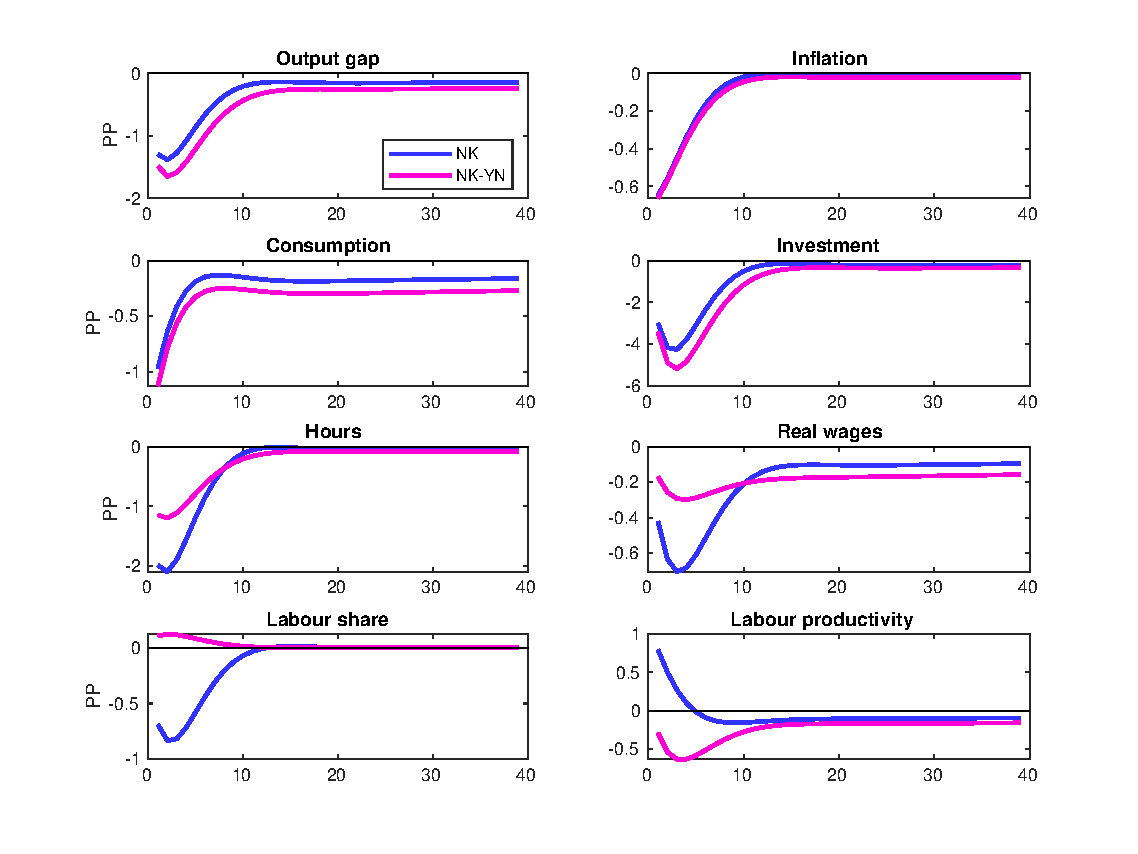
\includegraphics[width=14cm]{IRF_RANK.pdf}
\caption*{\RaggedRight \footnotesize Note: Figure shows response of selected aggregate variables to a 100 basis point monetary policy shock over an initial 40 quarters. Variables are expressed as percentage point deviations from steady state. NK refers to the response of an economy with only production labour and NK-YN is the response of a similarly calibrated economy with the inclusion of expansionary labour as described in section 2.}
\end{figure}

\subsubsection{WCNK}

\begin{figure}
\centering
\caption{\label{fig:IRF_WCNK}  - IRF to a monetary policy shock.}
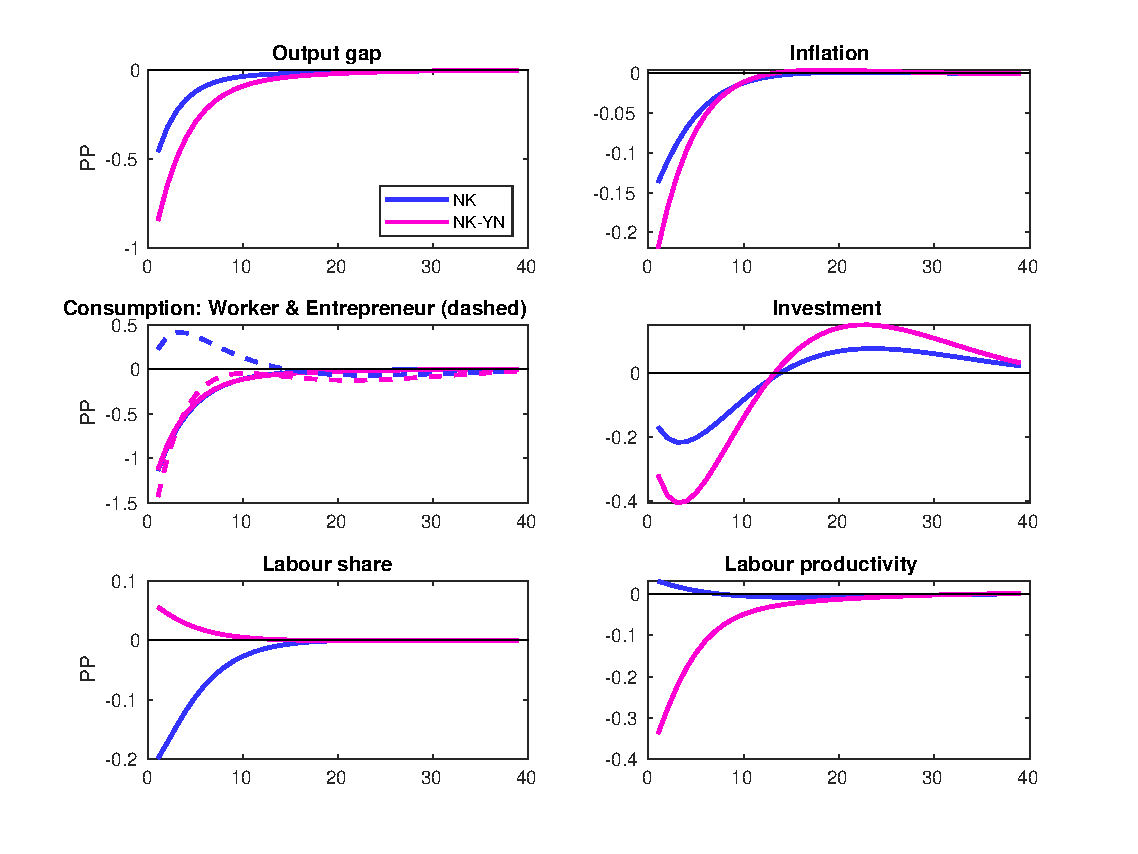
\includegraphics[width=14cm]{IRF_WCNK.pdf}
\caption*{\RaggedRight \footnotesize Note: Figure shows response of selected aggregate variables to a 100 basis point monetary policy shock over an initial 40 quarters. Variables are expressed as percentage point deviations from steady state. NK refers to the response of an economy with only production labour and NK-YN is the response of a similarly calibrated economy with the inclusion of expansionary labour as described in section 2.}
\end{figure}

\subsubsection{HANK}

\begin{figure}
\centering
\caption{\label{fig:IRF_HANK} HANK - IRF to a monetary policy shock.}
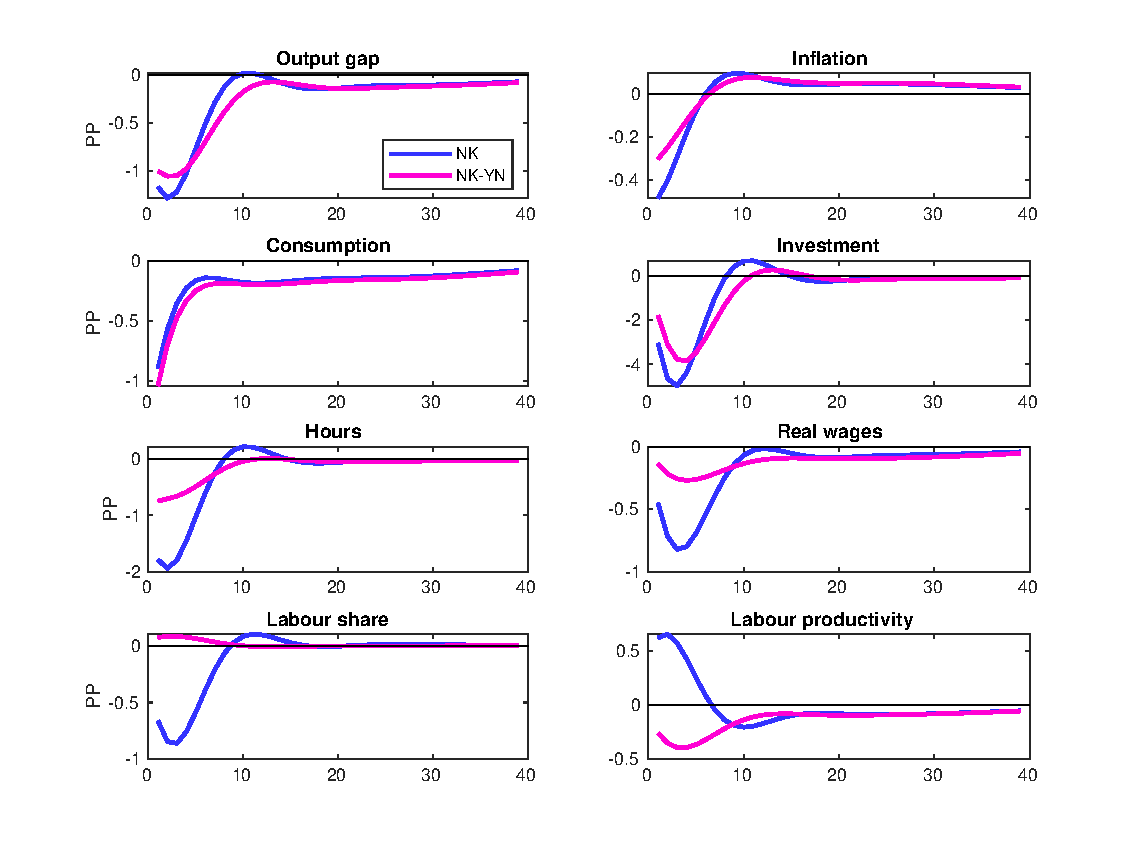
\includegraphics[width=14cm]{IRF_HANK.pdf}
\caption*{\RaggedRight \footnotesize Note: Figure shows response of selected aggregate variables to a 100 basis point monetary policy shock over an initial 40 quarters. Variables are expressed as percentage point deviations from steady state. NK refers to the response of an economy with only production labour and NK-YN is the response of a similarly calibrated economy with the inclusion of expansionary labour as described in section 2.}
\end{figure}

%%%%%%%%%%%%%%%%%%%%%%%%%%%%%%%%%%%%%%%%%%%%%%%%%%%%%%%%%%%%%%%%%%%%%%%%%%%%%%%%%%%%%%%%%%%%%%%%%%%%
%%%%%%%%%%%%%%%%%%%%%%%%%%%%%%%%%%%%%%%%%%%%%%%%%%%%%%%%%%%%%%%%%%%%%%%%%%%%%%%%%%%%%%%%%%%%%%%%%%%%%%

\section{Conclusion}



\newpage
\bibliography{sample}

\end{document}